\section*{Système proie-prédateur de Lotka-Volterra}

Dans cette partie, nous allons nous intéresser au système proie-prédateur de Lotka-Volterra, modélisant l'évolution de la population de plusieurs espèces dans un milieu naturel.
\vskip 1mm ~

Tout d'abord, nous allons étudier les modèles de de Malthus et Verhulst. Dans ces modèles, $N(t)$ décrit la variation de la population d'un ensemble d'individus au cours du temps. $b$ représente alors le taux de naissances et $d$ le taux de décès de la population. On a alors $\gamma =b-d$ et $\kappa$ qui représente la limite des ressources. Ainsi, on peut considérer que ces modèles représentent les variations d’une population.

Nous avons pu résoudre les équations différentielles de ces modèles à l'aide la méthode de Runge-Kutta d'ordre 4.
\vskip 1mm ~

Nous nous sommes ensuite intéressés au modèle de Lotka-Volterra, constitué de deux équations différentielles. Les paramètres $a$, $b$, $c$ et $d$ représentent respectivement le taux de reproduction des proies, le taux de mortalité des proies (dû aux prédateurs rencontrés), taux de reproduction des prédateurs en fonction des proies mangées et taux de mortalité des prédateurs. Ainsi, ce modèle permet bien de modéliser un écosystème proie/prédateur.

La figure~\ref{fig:lv1} représente les variations des deux populations au cours du temps et la figure~\ref{fig:lv2} représente les variations de $(N(t), P(t))$ au cours du temps. Les solutions de ce système sont périodiques.

\begin{figure}[ht]
	\centering
	\subfloat[Variation des populations $N$ et $P$ au cours du temps]{
		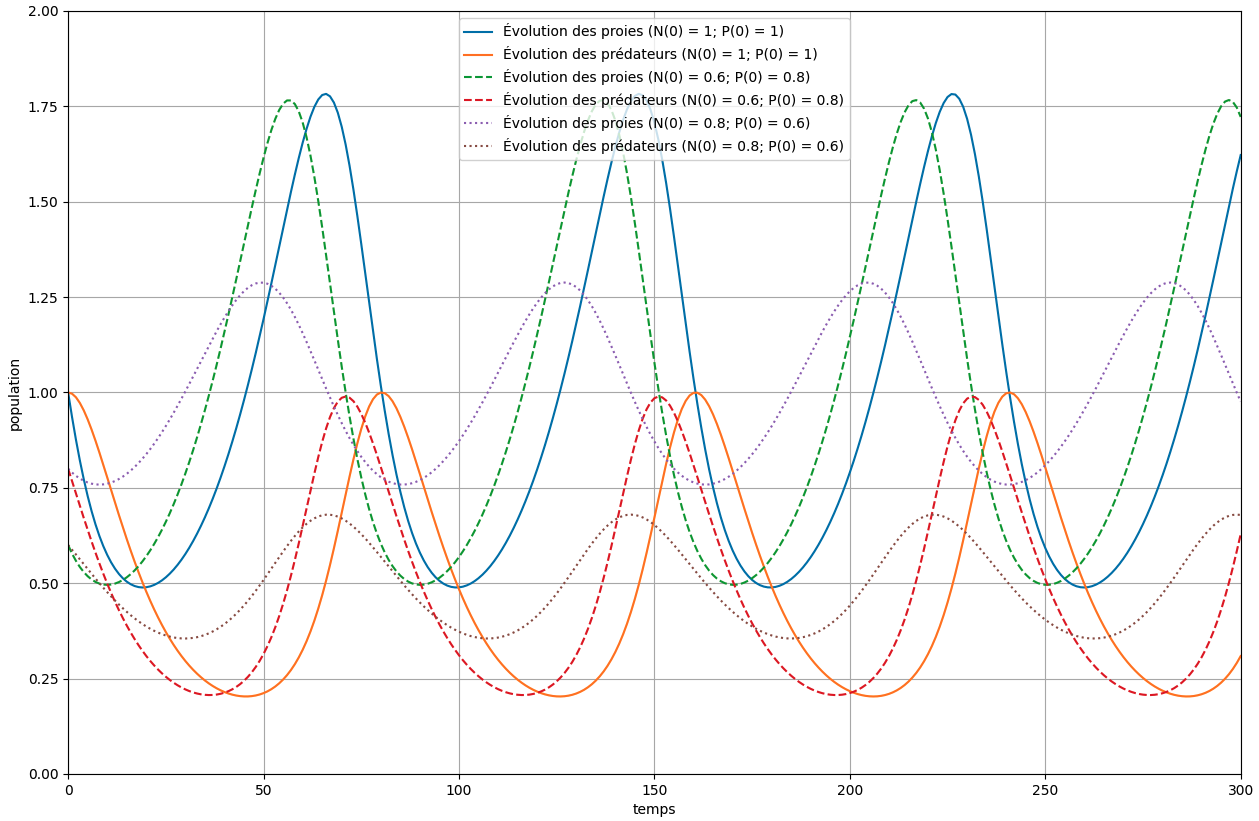
\includegraphics[width=0.55\textwidth]{img/lv1}
		\label{fig:lv1}
	}
	\subfloat[Variation de $(N(t), P(t))$ au cours du temps]{
		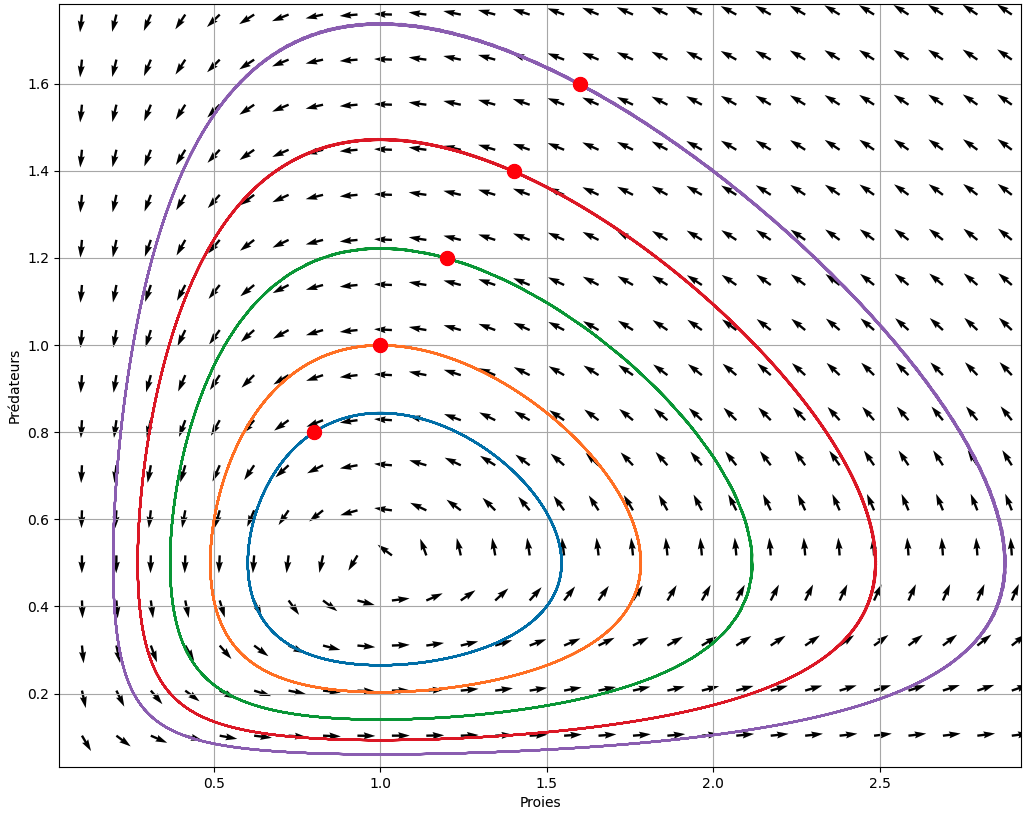
\includegraphics[width=0.44\textwidth]{img/lv2}
		\label{fig:lv2}
	}
	\caption{Résolutions du modèle de Lotka-Volterra avec différentes conditions initiales pour $a = \frac{2}{3}, b = \frac{4}{3}, c = 1 \text{ et } d =1$}
	\label{fig:lv}
\end{figure}

Les solutions étant périodiques, il est possible d'établir une estimation numérique de la période. Pour cela, nous cherchons deux maximums locaux successifs.
\vskip 1mm ~

On peut également étudier localement, sur la figure~\ref{fig:loc} les solutions autour d'un point de départ donné (ici $y_0 = [0.5,0.5]$). On remarque que les courbes des solutions ne se croisent pas.
\vskip 1mm ~

\begin{figure}[H]
	\centering
	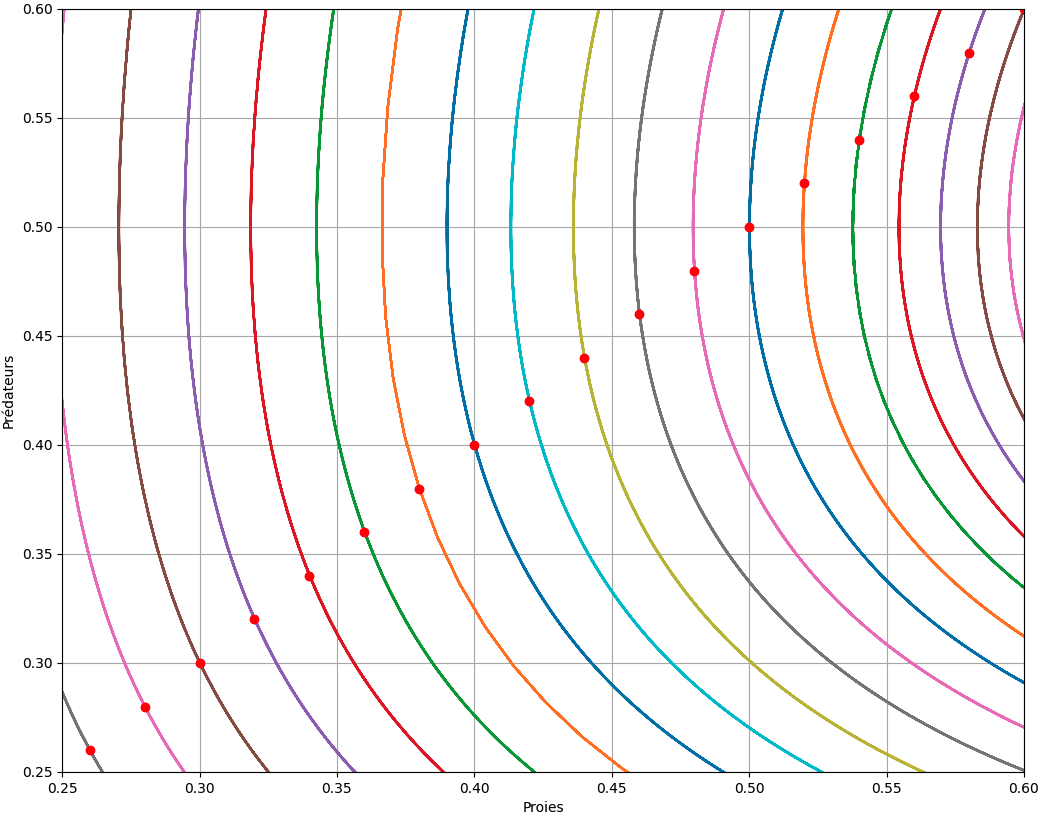
\includegraphics[width=0.5\textwidth]{img/loc}
	\caption{Étude locale de différentes solutions ayant des conditions initiales proches de $y_0 = [0.5,0.5]$}
	\label{fig:loc}
\end{figure}

Le système de Lotka-Volterra admet des points singuliers dès que les dérivées s'annulent. Ainsi, l'équation~\ref{eq:singular_points} décrit les points singuliers du système.

\begin{equation}
	\label{eq:singular_points}
	\begin{cases}
		a = bP(t)\\
		d = cN(t)
	\end{cases} \Leftrightarrow\quad
	\begin{cases}
		P(t) = \frac{a}{b} &(b \neq 0)\\
		N(t) = \frac{d}{c} &(c\neq 0)
	\end{cases}
	\quad\text{ et }\quad
	\begin{cases}
		P(t) = 0\\
		N(t) = 0
	\end{cases}
\end{equation}

Les diagrammes obtenus sont sous la forme d'orbites. Ceux-ci sont fermés. Si l'on part d'un point singulier, le système n'évolue pas. Le diagramme obtenu est alors un nuage des points singuliers.